% vim: et sw=2 ts=2 sts=2

\section{Métodos}
\frame{
\frametitle{Métodos}
\begin{block}{}
\begin{center}
  Como modelar a função $F$?
\end{center}
\end{block}
}

\frame{
\frametitle{Lógica Nebulosa (SAM)}
\begin{block}{}
  $$
    F(x) = \frac{\sum w_i.a_i(x).V_i.c_i}{\sum w_j.a_j(x).V_j}
  $$

  Com o volume/área $V_j$ e o centroide $c_j$ são dados por:

  $$
    V_j = \int{b_j(y_1,...,y_p)}_{\Re^{p}}.dy_1...dy_p > 0
  $$

  $$
    c_j = \frac{\int{y.b_j(y_1,...,y_p)}_{\Re^{p}}.dy_1...dy_p}{V_j}
  $$
  \end{block}
}

\frame{
\frametitle{Otimização da Colonia de Formigas}
\begin{block}{}
\subsection{Pseudo código da meta-heurística do ACO}
%Algoritmo
\begin{algorithm}[H]

  %Macros
  \SetKwBlock{AgendarAtividade}{AgendarAtividade}{fim}
  \SetKwBlock{Procedimento}{Procedimento}{fim}

  \Procedimento{
    \Enqto{$n < N_{MAX\_IT}$}{
      %\tcp*[f]{$N_{MAX\_IT}$ é o número máximo de iterações\\}
      \AgendarAtividade{
        ConstruirSolucoesFormigas\\
        AtualizarFeromonios\\
        %\tcp*[f]{opcional}\\
        \tcp{opcional:}
        AcoesGlobais
      }
    }
  }

  \caption{Pseudo código da meta-heurística do ACO}
\end{algorithm}
\end{block}
}

\frame{
\frametitle{Recozimento Simulado}
\begin{block}{}
  %Algoritmo
  \begin{algorithm}[H]
    %Macros
    \SetKwBlock{Procedimento}{Procedimento}{fim}

    \Procedimento{
      SetarValoresInicias\;
      EscolherVizinho\;

      CalcTransicao\;
      Atualizar Temperatura\;
    }

    \caption{Pseudo código da meta-heurística do SA}
  \end{algorithm}
\end{block}
}


\frame{
\frametitle{Algoritmo Genético}
\begin{block}{}
\subsection{Pseudo código de um Algorítimo Genético}

%\begin{lstlisting}
\begin{algorithm}[H]
\SetKwBlock{Procedimento}{Procedimento}{fim}

%Algorithm: GA(n, \ki, \mu)
\Procedimento{
  %// Initialise generation 0:
  $k \leftarrow 0$, $P_k \leftarrow n$ indivíduos aleatórios\;
  %// EvaluatePk:
  %\Para{cada $i$ em $P_k$}
  %Compute fitness(i) for each i ∈ Pk;
  %Computar a $avaliacao(i)$ para cada $i$ em $P_k$\;
  %while fitness of fittest individual in Pk is not high enough;
  %\Enqto{a $avaliacao(i)$ de cada $i$ em $P_k$ não for boa o suficiente}{
  \Enqto{$avaliacao(i) < desejado$ de cada $i$ em $P_k$}{
    %// Create generation k + 1:
    %// 1. Copy:
    %Select (1−χ)×n members ofPk and insert into Pk+1;
    Selecionar os $(1 - \chi) \times n$ membros com maior $avaliacao(i)$ de $P_k$ e inserir em $P_{k+1}$\;
    %// 2. Crossover:
    %Select χ×n members of Pk; pair them up; produce offspring; insert the offspring into Pk+1;
    Selecionar $\chi \times n$ membros de $P_k$, pareá-los e inserir a cria em $P_{k+1}$\;
    %// 3. Mutate:
    %Select µ×n members of Pk+1; invert a randomly-selected bit in each;
    Selecionar os $\mu \times n$ membros de $P_{k+1}$ com maior $avaliacao(i)$ e inverter um bit aleatório de cada membro\;
    %// Evaluate Pk+1:
    %Compute fitness(i) for each i ∈ Pk;
    %Computar a $avaliacao(i)$ para cada $i$ em $P_{k+1}$\;
    %// Increment:
    %k := k + 1;
    $k \leftarrow k + 1$\;
  }
%return the fittest individual from Pk;ut your code here.
  \Retorna{membro $i$ em $P_k$ com maior $avaliacao(i)$}
}
\caption{Pseudo código de um Algoritmo Genético}
\end{algorithm}
\end{block}
}


\frame{
\frametitle{Redes Neurais}
\begin{block}{}
\begin{figure}[H]
\centering
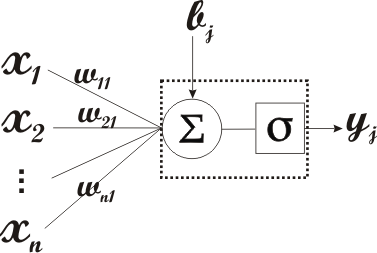
\includegraphics[width=10cm]{figuras/rede_neural_neuronio}
\caption{Modelo matemático de um neurônio.}
\end{figure}
\end{block}
}

\frame{
\frametitle{Redes Neurais}
\begin{block}{}
\begin{figure}[H]
\centering
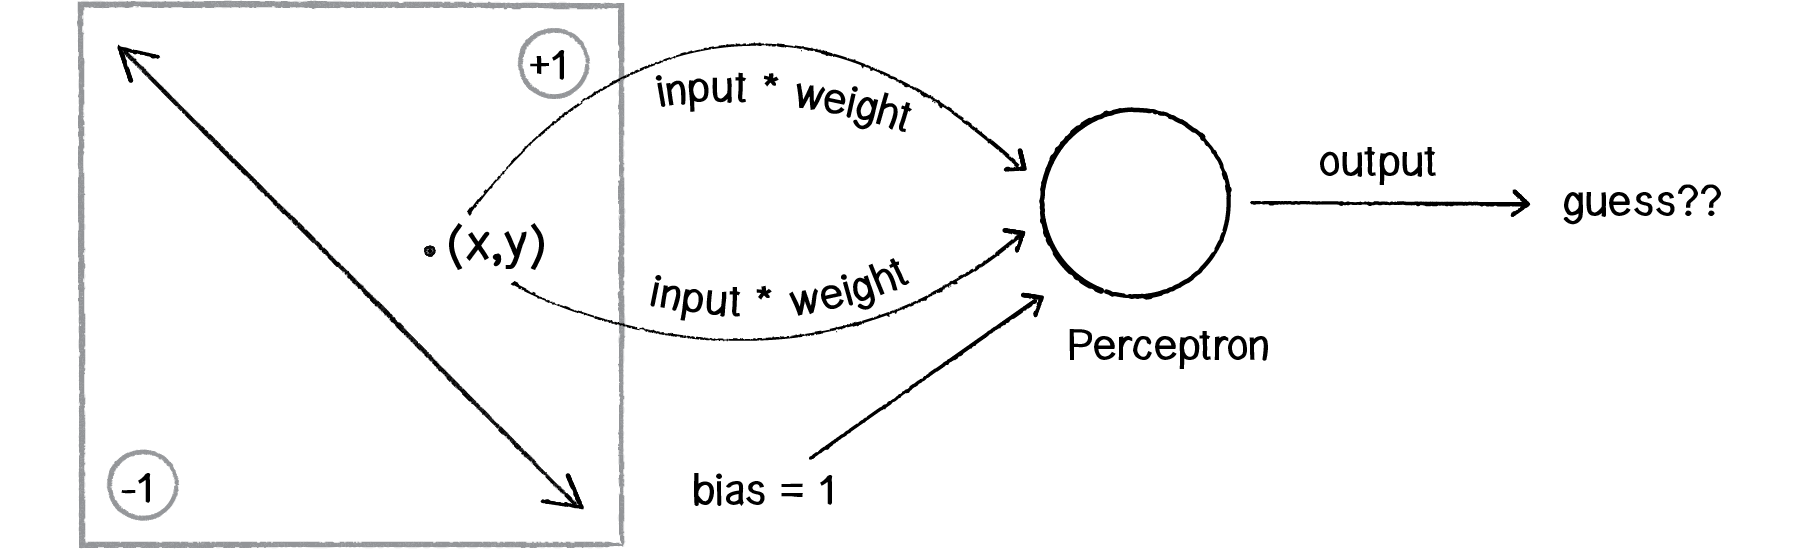
\includegraphics[width=10cm]{figuras/rede_neural_simple_problem}
\caption{\textit{Perceptron} para decidir região de um ponto no plano.}
\end{figure}
\end{block}
}

\frame{
\frametitle{Redes Neurais}
\begin{block}{}
\begin{figure}[H]
\centering
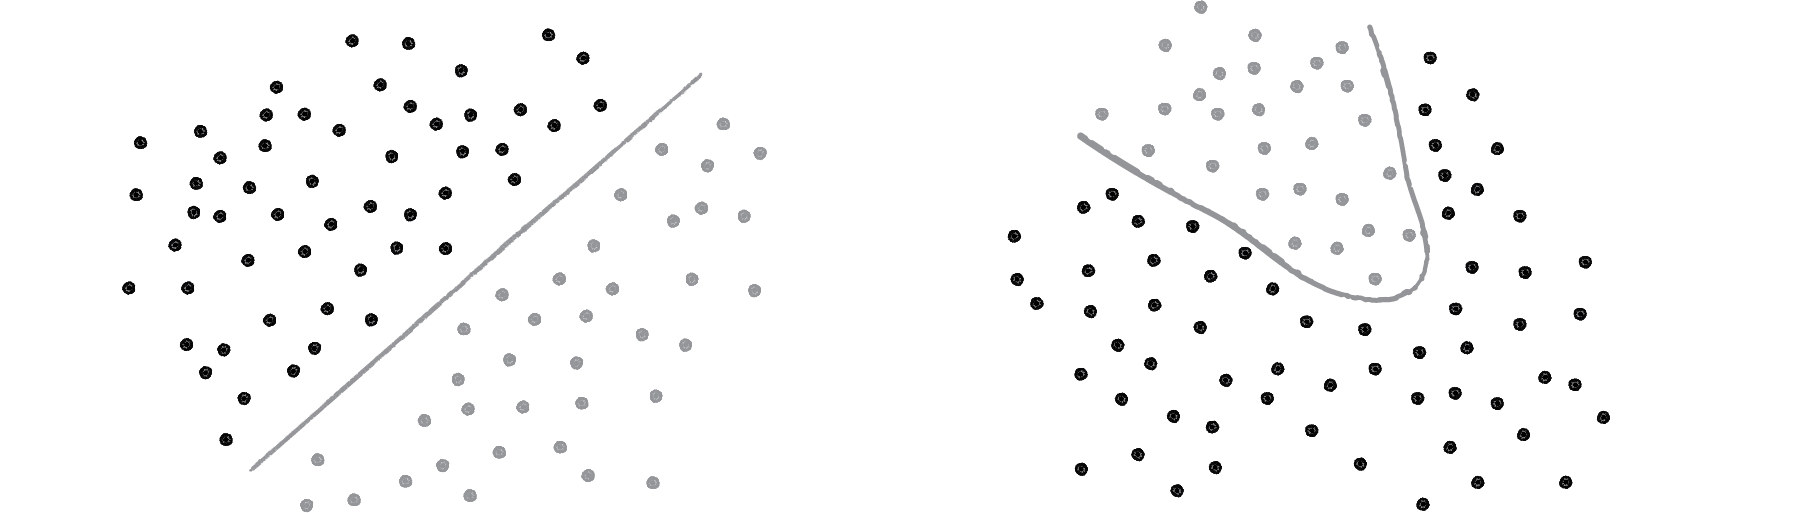
\includegraphics[width=10cm]{figuras/rede_neural_linear_probl}
\caption{Problemas linearmente separáveis vs. não linearmente separáveis.}
\end{figure}
\end{block}
}

\frame{
\frametitle{Redes Neurais}
\begin{block}{}
\begin{figure}[H]
\centering
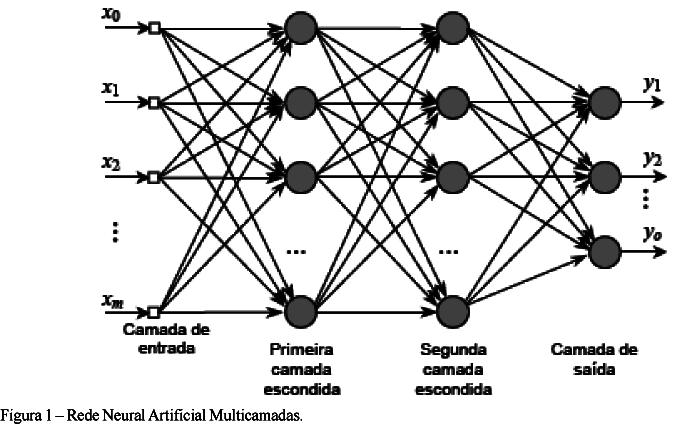
\includegraphics[width=8cm]{figuras/rede_neural_topologia}
\caption{Topologia de camadas.}
\end{figure}
\end{block}
}
